% !TEX root=../dymmy/dummy-04.tex

\chapter{双杂化泛函原子体系电子云密度与能量测评}
\label{sec.4.title}

\section{引言}

DFT 在 Hohenberg-Kohn 定理\cite{Hohenberg-Kohn.PR.1964}的框架下,是原理上严格的理论;即没有引入任何近似,且必然存在一个对所有体系普适、严格正确的泛函 $F[\rho]$;它可以导出精确的能量、电子云密度、各种分子或物质性质、以至于精确的波函数本身。

但现实是,我们难以获得严格的密度泛函 $F[\rho]$ 本身。依 Levy 的设想\cite{Levy-Levy.PNAS.1979},真实泛函需要在完整的波函数空间下作搜索,其代价是巨大的。更晚的讨论表明,所有 $k$-local Hamiltonian 问题 ($k > 2$) 与 $N$ 可表示问题是 QMA 的\cite{Kempe-Regev.SJC.2006, Liu-Verstraete.PRL.2007};进而 DFT 问题也是 QMA 的\cite{Schuch-Verstraete.NP.2009}。具体来说,普适泛函的计算消耗、泛函变量的空间两者总存在其一是 QMA 问题:
\begin{itemize}[nosep]
    \item 使用波函数 $\Psi$ 作为基本变量,而不用密度 $\rho(\bm{r})$ 描述;则由于过大的变量空间,计算消耗是 QMA 的 (Full-CI、QMC 或 Levy 约束搜索);
    \item 电子云密度 $\rho(\bm{r})$ 作为变量,则普适泛函 $F[\rho]$ 的计算消耗是 QMA 的;所有对 $F[\rho]$ 计算消耗将至 P (多项式复杂度) 的尝试都必然是近似 (DFT 理论);
    \item 若不使用单粒子密度 $\rho(\bm{r})$ 而使用双粒子密度 $\rho_2(\bm{r}, \bm{r}')$ 构造泛函,那么即使 $F[\rho_2]$ 的计算复杂度可能降至 P,但为限制双粒子密度 $\rho_2 (\bm{r}, \bm{r}')$ 在其定义域 ($N$ 可表示空间),其代价仍然是 QMA 的 (2-RDM 框架)。
\end{itemize}
因此,任何理论或实现框架都无法简单地解决分子或物质模拟问题。

但从具体实现上,DFT 理论近似的普适泛函 $F[\rho]$ 计算消耗小、且 $\rho(\bm{r})$ 作为变量的空间小,从而广受物质计算工作者的欢迎。而跨越构造普适泛函 $F[\rho]$ 的困难,则成为泛函开发者不懈的追求。

而在如何克服 $F[\rho]$ 构造上的困难,对其作有效的近似,不同的研究者持有不同的态度。一些研究者坚持对 $F[\rho]$ 的形式与性质作深入的研究;若了解愈多 $F[\rho]$ 的严格性质,就愈接近真实的严格普适泛函\cite{Kohn-Sham.PR.1965, Slater-Slater.PR.1951, Vosko-Nusair.CJP.1980, Perdew-Ernzerhof.PRL.1996, Adamo-Barone.JCP.1999, Ernzerhof-Scuseria.JCP.1999, Tao-Scuseria.PRL.2003, Cohen-Yang.CR.2012, Su-Xu.JCP.2014, Sun-Perdew.PRL.2015, Medvedev-Lyssenko.S.2017}。
另一些研究者在承认可预见的未来内 $F[\rho]$ 难以精确地构造的基础上,着重于更准确地描述具体的、当前物质科学所关心的问题;愈多类型的体系与性质可以被精确地描述,就愈接近真实的严格普适泛函\cite{Becke-Becke.PRA.1988, Lee-Parr.PRB.1988, Becke-Becke.JCP.1993, Zhao-Truhlar.JCP.2006, Grimme-Grimme.JCP.2006, Zhao-Truhlar.TCA.2008, Zhang-Goddard.PNAS.2009, Chai-Head-Gordon.JCP.2009, Zhang-Goddard.PNAS.2011, Zhang-Xu.JCP.2012, Yu-Truhlar.JCP.2016, Chen-Weinan.JCTC.2021}。

表面上,这两种看法的差异在于构造 $F[\rho]$ 时,是否存在经验参数。一般来说,前者通过严格性质构造 $F[\rho]$ 的途径,会使用较少甚至于没有经验参数。后者则通常对 $F[\rho]$ 作参数化;针对其所关心的物质计算问题,拟定数据训练集与验证集,对参数化的 $F[\rho]$ 作监督学习。而从实践的经验上,对于经验参数拟合的泛函,若计算问题处在训练集或验证集中,则通常有优异的表现;但若超出这些数据集的范围,则其表现很有可能因过拟合现象而粗强人意。相比之下,非经验参数拟合的泛函更有可能在各种物质及其性质上有良好的表现。

目前常用的密度泛函近似中,大多数都带有经验参数;而这些经验参数通常是针对能量性质的数据集而优化的。Medvedev 等\cite{Medvedev-Lyssenko.S.2017}指出,目前绝大多数泛函开发者关注于更精确地描述物质能量;其中不乏声音认为对能量更好的描述,可以给出更精确地泛函。但另一方面,电子云密度 $\rho(\bm{r})$ 作为密度泛函 $F[\rho]$ 的参量,作为连接多电子体系与能量的关键桥梁,却很少被关注到。基于对轻原子与正离子体系的电子云密度系统性的分析与测评,Medvedev 等认为,依泛函提出的年代顺序,2000 年以前发展的泛函在电子云密度上的表现较好、展现出 DFT 理论与其近似的进步;但 2000 年以后发展的泛函中,一部分泛函由于物理上不满足严格的性质、以及过分宽松的多经验参数拟合,使得后来的部分泛函在电子云密度的总体表现上逐年次第劣化。注意到密度泛函近似的目标是逼近普适泛函,而普适泛函应当能对所有的物质性质作精确的模拟;电子云密度作为密度泛函的重要物理量,当然并不例外。因此,对于这部分泛函,Medvedev 等人无法认同它们正在逼近普适泛函的道路上。同时他们认为,对于非参数或少量经验参数拟合的另一部分泛函,电子云密度确实地随“Jacob 阶梯”\cite{Perdew-Schmidt.ACP.2001}的爬升而愈加精确。

对于 Medvedev 等人的工作,不同的研究者表达过不同的看法。在 Kepp 的评论\cite{Kepp-Kepp.S.2017}中,其中一个重要的着眼点是:$F[\rho]$ (或者引入外势后的 $E[\rho]$) 作为泛函,它是 $\rho(\bm{r})$ 作为宗量到能量值作为应变量的映射;只有宗量与应变量两者都能描述好,近似的泛函才能认为真正地走在正确的道路上。同时,Kepp\cite{Kepp-Kepp.S.2017} 与王颖等人\cite{Wang-He.JCTC.2017} 对评价标准,特别是关于涉及 $\nabla^2 \rho(\bm{r})$ 的径向函数 LR 与基组选取的问题上有针对性的深入研究。

而对于双杂化泛函,特别是 xDH 型泛函\cite{Zhang-Goddard.PNAS.2009},其一方面在“Jacob 阶梯”的顶端,原则上通过这些信息可以精确的描述真实泛函的性质。它同时包含非局域交换 (严格交换能) 与相关效应 (以 MP2 型相关能为典型);其基于 G\"orling-Levy 二阶微扰\cite{Goerling-Levy.PRB.1993, Goerling-Levy.PRA.1994}、且 xDH 型泛函在自洽场与能量两步计算都使用了包含完整的相关与交换信息,理论上有可靠的依据。另一方面,多数双杂化泛函含有少量的经验参数;这既能保证泛函在化学关心的问题上有良好的表现,但同时也不会轻易地过度拟合,而破坏泛函在训练集外的表现、以及对理论发展的偏离。因此我们期待,以 xDH 型泛函为代表的双杂化泛函,在除能量以外的其他训练集所没有涵盖到的性质上,也可能有良好的表现。

在本章与第 \alertref{sec.6.title} 章,我们将对上述猜测作验证。我们基于 Medvedev 等人的工作\cite{Medvedev-Lyssenko.S.2017},对双杂化泛函作较为系统地评测。我们将同时关注能量 $E$ 与密度 $\rho(\bm{r})$ 的表现,并对基组依赖性作简要的讨论。我们期望表明,双杂化泛函不仅在反应能量上有良好的表现\cite{Su-Xu.WCMS.2016, Goerigk-Grimme.PCCP.2017, Zhang-Xu.JPCL.2021, Santra-Martin.JPCL.2021};在原子体系的电离和电子云密度的表现上,也沿着“Jacob 阶梯”仍然走在正确的道路上。

\section{实现细节}

\subsection{计算体系与方法}

本工作所涉及的体系是 14 个原子或离子体系 (\ce{Be^0}, \ce{B^+}, \ce{B^3+}, \ce{C^2+}, \ce{C^4+}, \ce{N^3+}, \ce{N^5+}, \ce{O^4+}, \ce{O^6+}, \ce{F^5+}, \ce{F^7+}, \ce{Ne^0}, \ce{Ne^6+}, \ce{Ne^8+}) 的电子云密度与能量。这些体系均为 2 ($1s^2$)、4 ($1s^2 2s^2$)、10 ($1s^2 2s^2 2p^6$) 电子体系。

与 Medvedev 等人的工作\cite{Medvedev-Lyssenko.S.2017}一致地,对于非变分方法,电子云密度 $\rho (\bm{r})$ 均使用弛豫密度生成 (对于 xDH 型泛函弛豫密度以 $D_{\mu \nu}^\textsf{DH}$ 表示,参考式 (\alertref{eq.3.def.dh-resp-dm}))。测评过程所选用的基组是 aug-cc-pωCV5Z;对于使用到 RI 近似的情形,其辅助基组使用 \textsc{PySCF} 默认的自动生成方案。所有双杂化密度泛函选用经 \textsc{PySCF} 默认简化的 (120, 770) 格点积分,测评所用程序为 \textsc{PySCF} (ver 2.4.0) 与 \textsc{dh} (commit 80ca9e8);密度泛函计算使用到 \textsc{LibXC} (commit 2a8caee)。对于 CCSD 方法,其自洽场能量收敛限是 $10^{-11} \ \text{Hartree}$、CCSD 能量收敛限是 $10^{-9} \ \text{Hartree}$;其余方法的能量收敛限均为 $10^{-9} \ \text{Hartree}$。本工作中其他 post-HF 方法 (MP4(sdq)、MP3) 计算使用 \textsc{Gaussian 09} 实现\cite{Su-Xu.PNAS.2018}。

密度测评的参考值是 CCSD/aug-cc-pωCV5Z 下的弛豫密度;$1s^2 2s^2 \rightarrow 1s^2$ 过程电离能测评的参考值是经 HF 方法下 Douglas-Kroll 近似对相对论效应作矫正后的实验值\cite{Kepp-Kepp.S.2017, Douglas-Kroll.APY.1974, NIST.Atomic}。本工作也会对基组依赖性、RI 近似精度等问题作讨论;其具体的计算方法将在具体的讨论中展开。

本工作对 Medvedev 等人的工作\cite{Medvedev-Lyssenko.S.2017}和苏乃强等人的工作\cite{Su-Xu.PNAS.2018}所测评的泛函作重新计算与验证、并补充目前流行的双杂化泛函。由于 \textsc{PySCF} 目前不支持含 $\nabla^2 \rho(\bm{r})$ 的 meta-GGA,因此未对 B98 作测评;同时不支持多个长短程参数 $\mu$ 的泛函,因此不对 HISS 作测评。出于收敛困难,因此未对含有 G96 交换的泛函 (包括 Gill, GLYP, GOP, GP86, GPBE, GPW91, GPZ81, GVWN, GVWN1RPA)、以及 MVS 和 SCAN 泛函作测评。出于实现方式不一致,本工作不展示 X$\alpha$ 的测评结果。因此,在 Medvedev 等人测评的 128 个泛函中,本工作测评并汇报其中 114 个泛函。同时,我们将引入 15 个 2015 年以后发展的低阶 (“Jacob 阶梯”上 1--4 阶) 新泛函、以及 44 个双杂化泛函,即总共 173 个泛函近似,如图 \ref{fig.4.functionals-distribution} 所示。由于不同程序的实现差异,BC, M05, M05-2X, M06-2X, M06-HF, M06-L, M08-SO, M11-L, MN12-L, SOGGA11, SOP, τHTCH, xDH-PBE0 等泛函的结果与早先文献有数值上的略微差异,但不影响总体结论。

\begin{figure}[hp]
    \centering
    \includegraphics[width=0.6\textwidth]{assets/functionals-distribution.pdf}
    \caption[原子体系电子云密度与能量测评的泛函分类与数量示意]{本工作测评泛函的大致分类与数量示意图。}
    \label{fig.4.functionals-distribution}
\end{figure}

\subsection{径向函数与密度测评标准定义}

本工作所采用的测评标准与 Medvedev 等人的工作\cite{Medvedev-Lyssenko.S.2017}一致,通过分析密度格点的 RDF 以作评测。该 RDF 的坐标选取为以原子核为中心均匀分布的 0 -- 10 \AA 的 50000 个格点。

在特定密度矩阵 $D_{\mu \nu}$ 下,电子云密度 $\rho(\bm{r})$ 定义为
\begin{equation}
    \rho(\bm{r}) = \sum_{\mu \nu} D_{\mu \nu} \phi_{\mu} (\bm{r}) \phi_{\nu} (\bm{r})
\end{equation}
对于原子体系,上述函数仅与电子到原子核距离 $r$ 有关,因此上述密度也写为 $\rho(r)$。密度径向函数 RHO、梯度 GRD 与二阶梯度 LR 分别定义为
\begin{align}
    \text{RHO}(r) &= 4 \pi r^2 \rho(r) \\
    \text{GRD}(r) &= 4 \pi r^2 | \nabla \rho(r) | = 4 \pi r^2 \left| \frac{\partial \rho(r)}{\partial r} \right| \\
    \text{LR}(r) &= 4 \pi r^2 \nabla^2 \rho(r) = 4 \pi r^2 \frac{\partial^2 \rho(r)}{\partial r^2}
\end{align}
对于给定的性质 $P \in \{\text{RHO}, \text{GRD}, \text{LR}\}$、原子或离子 $a \in \{\ce{Be^0}, \ce{B^+}, \cdots, \ce{Ne^8+}\}$、以及泛函近似或 post-HF 方法 $f, g$,RMSD 误差定义为
\begin{equation}
    \text{RMSD}_{P, a, (f, g)} = \sqrt{\frac{1}{N} \sum_i^N \big(P_{a, f} (r_i) - P_{a, g} (r_i) \big)^2}
\end{equation}
其中 $N = 50000$ 为格点数。特别地,若参考值选为 $g = \textsf{CCSD}$,则简记 $\text{RMSD}_{P, a, f} = \text{RMSD}_{P, a, (f, \textsf{CCSD})}$。为了合理地将不同性质的误差作公平的对比,上述的 RMSD 误差将除以性质均值数 median RMSD,得到均值数归一后的方均误差 MNAE:
\begin{equation}
    \text{MNAE}_{P, a, (f, g)} = \frac{\text{RMSD}_{P, a, (f, g)}}{\text{median}_{P} \text{RMSD}_{P, a, (f, g)}}
\end{equation}
最后,通过对原子指标 $a$ 求取极大值或平均值,可以得到泛函或方法 $f$ 在性质 $P$ 上的表现:
\begin{align}
    \text{maxMNAE}_{P, (f, g)} &= \max_a \text{MNAE}_{P, a, (f, g)} \\
    \text{meanMNAE}_{P, (f, g)} &= \underset{a}{\text{mean}} \, \text{MNAE}_{P, a, (f, g)}
\end{align}

本工作的 median RMSD,对于 RHO (单位 $\text{e} \, \text{\AA}^{-1}$) 为 0.009943368,对于 GRD (单位 $\text{e} \, \text{\AA}^{-1} \, \text{Bohr}^{-1}$) 为 0.092398036,对 LR (单位 $\text{e} \, \text{\AA}^{-1} \, \text{Bohr}^{-2}$) 为 1.445110833\footnote{在 Medvedev 等人的工作\cite{Medvedev-Lyssenko.S.2017} 中,用于图片展示的 GRD 的单位是 $\text{e} \, \text{\AA}^{-2}$、LR 的单位是 $\text{e} \, \text{\AA}^{-3}$;但我们的验证认为其单位换算可能存在问题。尽管如此,由于实际用于衡量泛函或方法间误差与优劣的标准是无量纲的 maxMNAE 或 meanMNAE,因此物理单位的问题不影响结论与讨论。}。

\section{测评结果}

完整的测评结果参考附录的表 \ref{tab.4.full-atom-benchmark}。由于数据较多,后文将对该表格的结果作分析与讨论。

\subsection{依年代发展的总体表现}

\begin{figure}[!t]
    \centering
    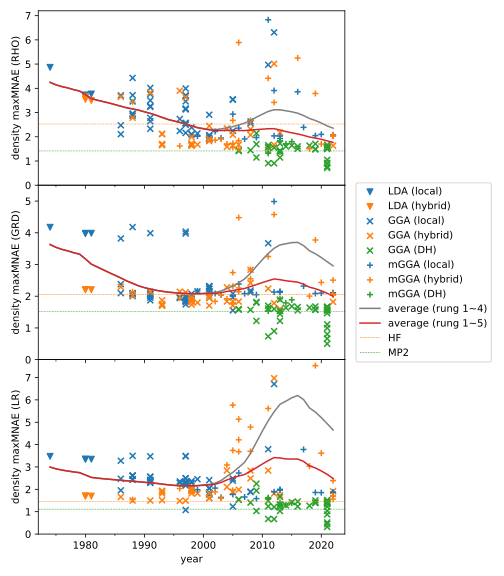
\includegraphics[width=0.8\textwidth]{assets/maxMNAE-against-year.pdf}
    \caption[径向函数 maxMNAE 对年代的散点图]{诸泛函密度径向函数最大均值数归一方均误差 (maxMNAE) 对其年代的散点图。实线表示的平均值曲线是通过对年代作 5 年为期的二次平均所得,因此反映的是前后 10 年左右的总体趋势变化。交换泛函中,局域部分所对应的泛函类型 (LDA、GGA、meta-GGA 或 mGGA) 以散点形状 (三角、叉号、加号) 区分;非局域部分 (无非局域、杂化、双杂化) 以颜色 (蓝色、橙色、绿色) 区分。由于部分数据点误差较大,在 GRD 图中 M11-L, N12, N12-SX, MN15, MN15-L 五个泛函、以及 LR 图中 M11-L, MN12-L, MN12-SX, MN15, MN15-L 五个泛函未展示在图中。}
    \label{fig.4.maxMNAE-against-year}
\end{figure}

Medvedev 等人工作的 Fig.\ 1 中,展现了随着年代的发展,泛函在密度径向函数 RHO 的测评上,平均误差在 2003 年左右先逐渐减小、尔后到 2015 年显著增大的情况。基于我们的测评,在图 \ref{fig.4.maxMNAE-against-year} 中,我们复现了这一趋势、并且对该图像作了拓展。图 \ref{fig.4.maxMNAE-against-year} 的灰色实线是“Jacob 阶梯”上低阶泛函依发展年代平均下密度径向函数的 maxMNAE 误差表现。相比于 Medvedev 等人的工作中,看到低阶密度泛函近似逐渐偏离正确结果的结论,我们看到误差在 2015 年达到高点以后逐渐下降的趋势。因此,从现在的眼光来看,低阶密度泛函近似确实回到了正确的道路上。

除此之外,我们补充了双杂化密度泛函近似的结果。图 \ref{fig.4.maxMNAE-against-year} 的红色实线体现了“Jacob 阶梯”上所有泛函近似依发展年代平均下密度径向函数的 maxMNAE 误差表现。Medvedev 等人的工作指出,在 2005 年以前,泛函近似大体上依“Jacob 阶梯”的爬升而在密度径向函数上的误差次第降低。而从图 \ref{fig.4.maxMNAE-against-year} 中,我们看到作为“Jacob 阶梯”上更高级别的方法,双杂化泛函相比于低阶泛函,其误差有显著的进一步降低。被测评的所有低阶泛函中,没有泛函在密度的表现上超越 MP2 方法;但不少双杂化泛函的表现相较于 MP2 更好。因此,尽管双杂化泛函付出了一定程度的计算代价,引入了对大体系而言计算量较大的 MP2 型相关能、以及对小体系而言计算量较大的密度泛函近似;但密度表现上有显著提升,同时好于低阶的泛函或 MP2 方法。

与此同时注意到,对于图 \ref{fig.4.maxMNAE-against-year},局域、杂化与双杂化泛函三个层级之间有较为明显的差别;但在每个层级内部,对于泛函是否掺杂 LDA、GGA 或 meta-GGA 形式的近似,影响不是非常显著。这表明,总体上来说,相比于引入局域信息仔细程度的多寡而言,泛函包含多少程度的非局域信息,将比较显著地影响泛函近似在密度上的测评结果。由于双杂化泛函同时包含了交换与相关两者的非局域效应,因此预期更有可能给出更好的密度表现。但同时需要指出,Medvedev 等人 Fig.\ 2 附近的讨论中,表明对于交换能,并非引入愈多的非局域杂化效应,密度上的表现愈好;引入适当的非局域效应才能正确描述密度性质。

除了密度性质外,在图 \ref{fig.4.MAE-etot-against-year} 中,我们也对诸泛函在离子体系 $1s^2 2s^2 \rightarrow 1s^2$ 过程电离能问题的表现作依泛函年代发展的测评。从年代的发展趋势来看,泛函近似的误差走势在原子电离能测评上与密度测评近乎一致,但细节的结构上有比较明显的不同。相比于密度的测评表现,对于原子的电离能,尽管一般来说包含愈多的非局域信息 (即泛函从“Jacob 阶梯”的第 1--3 阶爬升到第 4 到第 5 阶) 通常有愈稳定且愈低的误差,但这种优势并非是绝对的。事实上,如果仅从表现最优异的泛函来看,甚至结论是相反的:不含任何杂化的 PBELYP (MAE 误差 0.12 eV) 比杂化泛函 M06-2X (MAE 误差 0.23 eV) 比双杂化泛函 revXYG3 (MAE 误差 0.31 eV) 要更为精确。但一方面,误差较大的泛函通常是低阶泛函、而高阶泛函在电离能上的表现可以保证稳定地好于 HF 方法。而另一方面,对于低阶泛函,不少情形下可以对能量或密度的其中一者有良好的描述,但往往难以同时对两者都有出色的表现。以上面列举的三个泛函为例,若以 RHO、GRD、LR 三者的 maxMNAE 取最大值作为密度径向函数的测评标准,则 revXYG3 (1.113) 比 PBELYP (3.710) 比 M06-2X (4.214) 要更为出色。双杂化泛函确实不仅可以平衡能量和密度误差的表现,也可以对两者同时有相当精确的描述。

\begin{figure}[t]
    \centering
    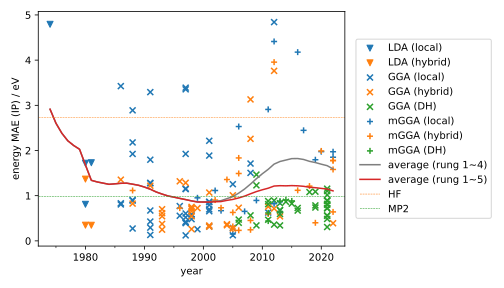
\includegraphics[width=0.7\textwidth]{assets/MAE-etot-against-year.pdf}
    \caption[电离能平均误差 MAE 对年代的散点图]{诸泛函电离能平均误差 MAE 对其年代的散点图。图例参考图 \ref{fig.4.maxMNAE-against-year}。}
    \label{fig.4.MAE-etot-against-year}
\end{figure}

\subsection{具体测评表现}

这里我们将更具体地讨论泛函的测评误差表现。

密度径向函数的测评包含三个指标,即 RHO ($\rho(\bm{r})$)、GRD ($|\nabla \rho(\bm{r})|$) 与 LR ($\nabla^2 \rho(\bm{r})$)。由于这些指标之间有比较强的相互关联,因此泛函在其中一个指标上的表现若更好,往往也在其他的指标上有不错的表现。图 \ref{fig.4.compare-err-RHO-GRD} 作为一个例子,对 RHO 与 GRD 的指标误差进行绘制,可以印证上述结论。同时注意到,相比于局域与杂化泛函而言,双杂化泛函在不同的密度径向函数误差指标上的一致性更强,即在图 \ref{fig.4.compare-err-RHO-GRD} 上代表双杂化泛函的散点更靠近黑色的实线。

\begin{figure}[t]
    \centering
    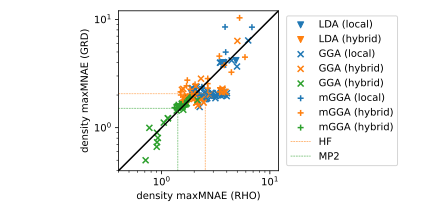
\includegraphics[width=0.6\textwidth]{assets/compare-err-RHO-GRD.pdf}
    \caption[密度径向函数 $\text{maxMNAE}_\text{RHO}$ 与 $\text{maxMNAE}_\text{GRD}$ 对照图]{诸泛函密度径向函数测评的 $\text{maxMNAE}_\text{RHO}$ 与 $\text{maxMNAE}_\text{GRD}$ 对照图。}
    \label{fig.4.compare-err-RHO-GRD}
\end{figure}

但类似的情况,对于电离能和密度径向函数的比较上并不成立。以图 \ref{fig.4.compare-err-maxMNAE-MAEIP} 为例,尽管大多数泛函大体上在当密度表现较好时,电离能的表现也较好;但注意到低阶的局域与杂化泛函中,不少在能量表现上优异、但在密度表现则稍差。图 \ref{fig.4.compare-err-maxMNAE-MAEIP} 中橙色虚线表示 HF 方法的误差;我们发现绝大多数能量误差最低的泛函 (包括 PBELYP (0.12 eV), mPWLYP1w (0.12 eV), PW91LYP (0.13 eV), TPSSLYP1w (0.15 eV), M06-2X (0.23 eV), M08-SO (0.25 eV) 等) 的密度误差显著地大于 HF 方法。一般来说,以 maxMNAE 为考察标准,重参数拟合的泛函如 M08-SO (4.78), M06-2X (4.21) 的误差要大于少参数或无参数泛函如 PBELYP (3.71), mPWLYP1w (3.53);这在 M11-L (16.27) 与 MN12-SX (13.00) 等泛函体现地更为明显。对于能量表现良好、但密度表现较差的泛函,我们认为这是由于密度 $\rho$ 的误差与能量泛函的误差 $E[\rho]$ 相互抵消所致;正确的结果不能因为两次错误恰好相互抵消,而就这样认为能量结果导出的过程便是正确的\cite{Hammes-Schiffer-Hammes-Schiffer.S.2017, Korth-Korth.ACIE.2017, Graziano-Graziano.NRC.2017};一旦泛函的优化方式有所改变,原本有可能正确的能量,很可能会产生严重的错误 (以电离能的 MAE 作为测评标准,尽管 M06-2X 误差很小,但其衍生发展的泛函误差相当大,其中 M11-L 误差 2.91 eV、MN12-SX 误差 3.96 eV)。而 B3LYPV1R (Gaussian 与 LibXC 默认的 B3LYP 方法,0.25 eV) 与 mPW1LYP (0.26 eV) 等泛函近似的密度误差 (以 maxMNAE 评测) 也小于 HF 方法;这些泛函在与 HF 方法计算量相当的前提下,可以认为有效地同时处理好密度与能量的计算。

\begin{figure}[t]
    \centering
    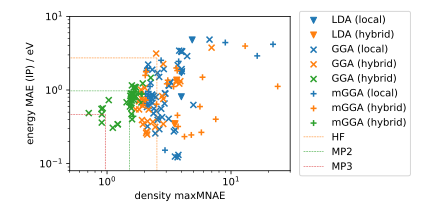
\includegraphics[width=0.6\textwidth]{assets/compare-err-maxMNAE-MAEIP.pdf}
    \caption[诸泛函密度径向函数 $\text{maxMNAE}$ 与电离能 MAE 对照图]{诸泛函密度径向函数测评的 $\text{maxMNAE}$ 与电离能的平均绝对值误差 (MAE) 对照图。这里的 maxMNAE 是指三个密度测评指标 $\text{maxMNAE}_\text{RHO}$、$\text{maxMNAE}_\text{GRD}$、$\text{maxMNAE}_\text{LR}$ 的最大值。}
    \label{fig.4.compare-err-maxMNAE-MAEIP}
\end{figure}

但我们同时注意到,目前没有任何低阶的局域与杂化泛函,在密度的表现上 (以 maxMNAE 评测) 可以优于 MP2 方法。这个情形不仅在 2015 年以前发展的低阶泛函成立,也在 2015 年以后发展的低阶泛函成立。但对于双杂化泛函而言,一方面不少泛函的密度与能量误差同时小于或接近 MP2 方法的级别;即使超出了 MP2 的误差,也通常不会大于 HF 方法的误差。因此,目前所有双杂化泛函的密度与能量都可以认为比较可靠。另一方面,revXYGJ-OS, XYG6, xDH-PBE0, XYGJ-OS, XYG5 等五个泛函的能量与密度的表现甚至超越了 MP3 方法;因此,双杂化泛函有希望以较低的代价,同时在密度与能量的表现上逼近计算量更为庞大的波函数方法。

\begin{figure}[t]
    \centering
    \includegraphics[width=0.6\textwidth]{assets/compare-err-maxMNAE-MAEIP-dh.pdf}
    \caption[双杂化泛函密度径向函数 $\text{maxMNAE}$ 与电离能的 MAE 对照图]{双杂化泛函密度径向函数测评的 $\text{maxMNAE}$ 与电离能的平均绝对值误差 (MAE) 对照图。这里的 maxMNAE 是指三个密度测评指标 $\text{maxMNAE}_\text{RHO}$、$\text{maxMNAE}_\text{GRD}$、$\text{maxMNAE}_\text{LR}$ 的最大值。}
    \label{fig.4.compare-err-maxMNAE-MAEIP-dh}
\end{figure}

在双杂化泛函中,xDH 型泛函的表现与 bDH 型泛函的表现也有所差异。图 \ref{fig.4.compare-err-maxMNAE-MAEIP-dh} 与图 \ref{fig.4.compare-err-maxMNAE-MAEIP} 相同,但仅绘制双杂化泛函的数据,并区分 xDH 型与 bDH 型泛函。可以看到,xDH 型泛函不仅在能量、也同时在密度上,有着比 bDH 型泛函更优异的表现。在 bDH 型泛函中,仅有 DSD-PBEPBE-D3BJ 与 DSD-PBEB95-D3BJ 相较于 MP2 而言有更优异的密度与能量表现;但除 XYG7 外的所有测评的 xDH 型泛函,其表现都优于 MP2 方法,且也与 DSD 系列泛函拉开了一定的差距。

\section{讨论与本章小结}

\begin{figure}[t]
    \centering
    \includegraphics[width=0.9\textwidth]{assets/compare-err-relative.pdf}
    \caption[部分泛函密度径向函数 maxMNAE 与电离能 MAE 测评表现示意图]{部分泛函的密度径向函数最大误差 maxMNAE 与电离能平均绝对误差 MAE 测评表现示意图。线图 (maxMNAE) 的误差是指三个密度测评指标 $\text{maxMNAE}_\text{RHO}$、$\text{maxMNAE}_\text{GRD}$、$\text{maxMNAE}_\text{LR}$ 的最大值。柱状图 (电离能误差) 的零点选取为 MP2 的误差 (0.973 eV)。对于特定泛函近似,只有其在图上对应的条形柱与散点都在红色五角星标识的 MP2 误差的情形下,该方法才能被认为同时在电离能与密度径向函数的表现上都优于 MP2 方法。}
    \label{fig.4.compare-err-relative}
\end{figure}

上面的结果分析,确实地验证了当前双杂化泛函、特别是 xDH 型双杂化泛函,在原子体系的电离能与电子云密度上有良好的表现。作为具体的例子,部分泛函的测评结果用更加直观的方式,呈现在图 \ref{fig.4.compare-err-relative} 中。需要注意到,所有本章涉及到的密度泛函,都并未专门针对这些测评标准所优化;因此几乎不存在因为经验参数拟合而有更好表现的可能——良好的测评表现更适合归因于泛函本身的优势。

Medvedev 等人的工作也已经表明,除了少数特定的泛函,泛函的“Jacob 阶梯”越高、电子云密度表现越好。我们注意到特别在电子云密度的表现上,作为“Jacob 阶梯”上最高的类别,双杂化泛函相比于其他泛函都有明显的优势;从而我们的工作印证并延伸了 Medvedev 等人的结论。因此,对于 xDH 型泛函,其优势之一在于它是“Jacob 阶梯”最高阶的双杂化泛函。

而其优势之二在于,它提供了一种切实可行、易于实现的同时矫正能量与密度误差的方案。现在一种普遍接受与流行的观点是,密度泛函近似存在两个误差来源:一是能量驱动误差、二是密度驱动误差。一般来说,能量驱动误差更为关键\cite{Cohen-Yang.CR.2012};但在一些的情况下,密度驱动的误差也会产生重要的影响\cite{Kim-Burke.JCP.2014}。事实上,这两种误差在标准的 Kohn-Sham 框架下是相互耦合的:欠佳的交换相关泛函将会给出欠佳的能量;而对这个欠佳的能量作变分,将会给出偏离真实的 Kohn-Sham 势函数,进而无法给出真实精确地密度。因此,能量与密度通过 Kohn-Sham 势函数得以联系起来:
\begin{equation}
    v_\textmt{xc} (\bm{r}) = \frac{\delta E_\textmt{xc} [\rho]}{\delta \rho(\bm{r})}
\end{equation}
或者在 Generalized Kohn-Sham 理论下,将 $E_\textmt{xc}$ 看作双粒子密度的泛函 (而并非是局域的关于 $\bm{r}$ 函数的泛函) 时,能量与密度通过下述势函数得以联系:
\begin{equation}
    v_\textmt{xc}^\mathrm{GKS} (\bm{r}, \bm{r}') = \frac{\delta E_\textmt{xc}}{\delta \rho(\bm{r}, \bm{r}')}
\end{equation}
后者实际上已经突破了 Kohn-Sham 理论框架本身了\cite{Su-Xu.WCMS.2016, Su-Xu.IJQC.2015, Su-Xu.MP.2016}。对于“Jacob 阶梯”上第五阶泛函,它并非表示为密度 $\rho(\bm{r})$ 或密度矩阵 $D_{\mu \nu}$ 的显式泛函;而这应当是真实泛函的特征\cite{Kohn-Kohn.PRB.1986, Yang-Mori-Sanchez.JCP.2012}。对于 xDH 型泛函,其使用较低阶的泛函近似,大体上可信与精确、但同时又以良好效率性价比地给出密度与轨道信息;而同时,在最终能量计算时,则引入更高阶的双杂化泛函近似形式,以通过引入非局域相关能效应 (也是 GKS 框架下泛函应当具有的特性) 的方式,进一步提升能量计算的精度。低阶泛函自洽场的电子云密度,则可以通过高阶能量泛函相对于自洽场泛函之差所给出的微扰,以 Z-Vector 方法矫正\cite{Handy-Schaefer.JCP.1984, Su-Xu.JCC.2013}。相比之下,低阶泛函所包含的非局域信息不足;而 bDH 型泛函则在自洽场泛函中没有引入完整的相关效应,因此自洽场所给出的密度也缺失一些相关效应。正因为 xDH 型泛函近似在框架设计上克服了上述两类泛函的困难,可以对能量与密度两者分别作精度的调整与提升;从而,xDH 型泛函近似相比于其他低阶泛函近似、以及 bDH 型双杂化泛函近似,更有可能同时在能量与密度上有良好的表现。

对于低阶泛函普遍逊色于高阶泛函、特别是 xDH 型泛函;我们作如下理解。从分数电荷的表现上,xDH 型泛函表现显著地好于传统泛函\cite{Su-Xu.IJQC.2015, Su-Xu.WCMS.2016, Su-Xu.MP.2016, Su-Xu.ARPC.2017},即更接近 PPLB 定理所要求的直线型分数电荷电离趋势\cite{Perdew-Balduz.PRL.1982}。作为第四阶的杂化泛函,分数电荷表现欠佳;这可以归因于非局域的严格交换效应没有很好地被非局域的相关效应所平衡;而 MP2 型相关效应,作为一种非局域相关效应,其引入可以很大程度上缓解分数电荷的计算误差。分数电荷在概念上与电子云有密切的联系,因此上述讨论,很可能适用于对以 xDH 型泛函为代表的双杂化泛函,在密度表现上断档式地好于低阶泛函,这种现象的一种解释。

作为展望,“Jacob 阶梯”不仅是对现有的泛函近似的一种归类方式,同样也是对未来泛函发展思路的一种指导。一方面,对于分子体系计算,从泛函近似的发展上、或从计算可行性上,引入严格交换能已经成为比较普遍的共识;因此,如果泛函近似还有哪些不足,则应该认为在相关贡献上有更多文章可作。为拓展泛函近似的可能性,作为一条前进的道路,在本论文的第 \alertref{sec.2.title} 章中,我们尝试了在双杂化框架下引入成对电子型相关能,以避免 MP2 型相关能在 HOMO/LUMO gap 过小的体系的误差。我们也期待在“Jacob 阶梯”的最高阶上有更多的工作,以拓展双杂化泛函的应用范围,在计算量可接受的方法与算法下,其能量与性质越来越接近普适泛函、达到梦想的化学精度。
